\subsection{位姿估计与场景管理模块}
\par 该模块以\texttt{Viewer}类(见表\ref{table:Viewer})和\texttt{Space}类(见表\ref{table:Space})为主体,分别负责相机位姿的管理和场景空间点云数据的管理,组件图如图\ref{fig:component2}所示。
系统通过\texttt{ManageData}函数实现CPU与GPU之间的数据交换与管理。由于系统设计多线程编程,需要使用锁机制防止资源冲突,保证数据的同步和并发。

\begin{figure}[htb]
	\centering
	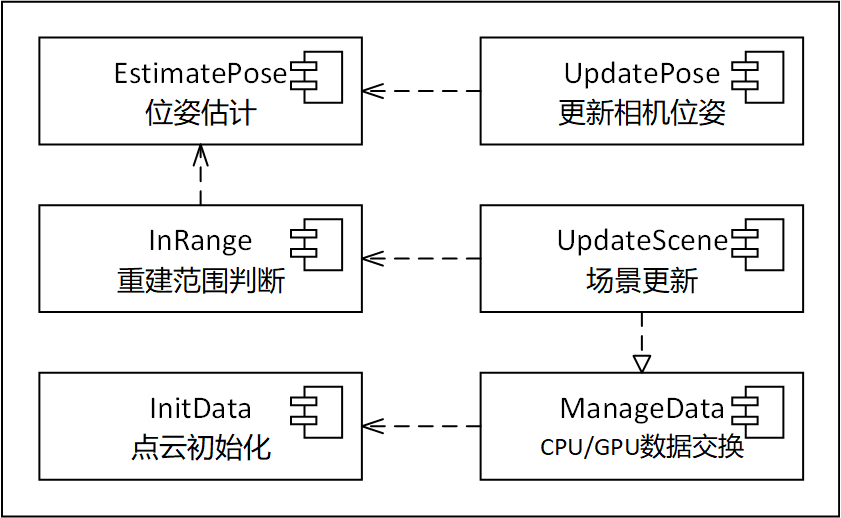
\includegraphics[width=0.7\textwidth]{figures/uml/component2.png}
	\caption{位姿估计与场景管理模块组件图}
	\label{fig:component2}
\end{figure}

\par 首先,位姿估计的任务由\texttt{Viewer}类的成员函数\texttt{EstimatePose}完成。当数据采集模块获得一帧新
的RGB-D数据,即\texttt{curr\_frame}后,利用对极几何原理,根据前一帧数据\texttt{old\_frame}
与\texttt{curr\_frame}之间的连续性和一致性,计算出当前相机的位姿矩阵并转换为一维数组存储到\texttt{pose}中:
\begin{align}
	T_{cam} & =
	\begin{bmatrix}
		R   & t \\
		0^T & 1
	\end{bmatrix}
	=
	\begin{bmatrix}
		\texttt{pose[0]}  & \texttt{pose[1]}  & \texttt{pose[2]}  & \texttt{pose[3]}  \\
		\texttt{pose[4]}  & \texttt{pose[5]}  & \texttt{pose[6]}  & \texttt{pose[7]}  \\
		\texttt{pose[8]}  & \texttt{pose[9]}  & \texttt{pose[10]} & \texttt{pose[11]} \\
		\texttt{pose[12]} & \texttt{pose[13]} & \texttt{pose[14]} & \texttt{pose[15]}
	\end{bmatrix}
\end{align}

\par 其中,$R$是 $3 \times 3$ 的旋转矩阵,$t$是 $3 \times 1$ 的平移向量。因此,对于相机坐标系中的点$P_{cam}$,可以通过公式\ref{pose_matrix}
计算出其在世界坐标系中对应的坐标 $P_w$:
\begin{equation*}
	\text{令}P_w =
	\begin{bmatrix}
		x_w \\
		y_w \\
		z_w
	\end{bmatrix}\text{,}
	P_{cam} =
	\begin{bmatrix}
		x_{cam} \\
		y_{cam} \\
		z_{cam}
	\end{bmatrix}
\end{equation*}

\par 于是,相机坐标系到世界坐标系的转换为:

\begin{equation}
	\begin{bmatrix}
		P_w \\
		1
	\end{bmatrix}
	= T_{cam}
	\begin{bmatrix}
		P_{cam} \\
		1
	\end{bmatrix}
	=
	\begin{bmatrix}
		R   & t \\
		0^T & 1
	\end{bmatrix}
	\begin{bmatrix}
		P_{cam} \\
		1
	\end{bmatrix}
	=
	\begin{bmatrix}
		RP_{cam} + t \\
		1
	\end{bmatrix}
	\label{pose_matrix}
\end{equation}

\par 位姿矩阵将为后续的三维重建提供基本的空间信息。一旦计算出位姿矩阵,就可以通过\texttt{UpdatePose}将相机位置和朝向信息更新到\texttt{Viewer}类中,供可视化模块使用。

\begin{table}[htb]
	\centering
	\caption{Viewer类的主要成员和方法}
	\label{table:Viewer}
	\begin{tabular}{|l|m{4cm}|m{3cm}|m{5cm}|}
		\hline
		                    & \multicolumn{1}{c|}{名称}                   & \multicolumn{1}{c|}{类型}          & \multicolumn{1}{c|}{功能}                         \\ \hline
		\multirow{7}{*}{成员} & \centering\arraybackslash intrinsic       & \centering\arraybackslash Matrix & \centering\arraybackslash 相机内参                  \\ \cline{2-4}
		                    & \centering\arraybackslash pose            & \centering\arraybackslash Matrix & \centering\arraybackslash 当前相机的位姿               \\ \cline{2-4}
		                    & \centering\arraybackslash position{[}3{]} & \centering\arraybackslash float  & \centering\arraybackslash \multirow{3}{*}{相机朝向} \\ \cline{2-3}
		                    & \centering\arraybackslash front{[}3{]}    & \centering\arraybackslash float  & \centering\arraybackslash                       \\ \cline{2-3}
		                    & \centering\arraybackslash gaze{[}3{]}     & \centering\arraybackslash float  & \centering\arraybackslash                       \\ \cline{2-4}
		                    & \centering\arraybackslash curr\_frame     & \centering\arraybackslash Frame  & \centering\arraybackslash 当前帧                   \\ \cline{2-4}
		                    & \centering\arraybackslash old\_frame      & \centering\arraybackslash Frame  & \centering\arraybackslash 上一帧                   \\ \hline
		\multirow{2}{*}{方法} & \centering\arraybackslash EstimatePose    & \centering\arraybackslash void   & \centering\arraybackslash 位姿估计                  \\ \cline{2-4}
		                    & \centering\arraybackslash UpdatePose      & \centering\arraybackslash void   & \centering\arraybackslash 更新相机位置和朝向             \\ \hline
	\end{tabular}
\end{table}

\par 在获得第一帧图像之前,模块首先实例化一个\texttt{Space}对象来管理场景空间和点云数据。系统先调
用\texttt{InitData}函数初始化点云数据,设定空间的原点坐标,设置场景重建的范围和点之间的距离,以
及\texttt{Point}结构体类型(见表\ref{table:point})的点云数组,包含每个点的坐标、RGB、类别标签等信息。

\begin{table}[htb]
	\centering
	\caption{Point结构体的成员}
	\begin{tabular}{cm{2.2cm}m{2.2cm}m{2.2cm}m{2.2cm}m{2.2cm}}
		\toprule
		名称 & \centering\arraybackslash x        & \centering\arraybackslash y     & \centering\arraybackslash z            & \centering\arraybackslash color\_b & \centering\arraybackslash color\_g      \\
		类型 & \centering\arraybackslash float    & \centering\arraybackslash float & \centering\arraybackslash float        & \centering\arraybackslash float    & \centering\arraybackslash float         \\
		\midrule
		名称 & \centering\arraybackslash color\_r & \centering\arraybackslash tsdf  & \centering\arraybackslash tsdf\_weight & \centering\arraybackslash label    & \centering\arraybackslash label\_weight \\
		类型 & \centering\arraybackslash float    & \centering\arraybackslash float & \centering\arraybackslash float        & \centering\arraybackslash int      & \centering\arraybackslash float         \\
		\bottomrule
	\end{tabular}
	\label{table:point}
\end{table}

\par 在场景管理过程中,系统在逻辑上将三维空间划分为四分之一重叠空间网格。\texttt{EstimatePose}计算出每一帧的
位姿矩阵后,首先调用\texttt{InRange}确定新的图像中的重建空间是否在当前的网格内,该
函数根据当前相机位姿进行判断。如果新的重建空间在当前的网格内,则进入点云生成与语义融合操作;如
果超出了范围,则需要进行场景更新。

\par 场景更新通过调用\texttt{UpdateScene}函数实现。首先,该函数调用\texttt{ManageData},将GPU中的点云数据
拷贝回CPU的点云数组中,调用模型导入导出模块,根据坐标所在的网格位置将点云模型保存为数据
文件。然后根据相机的位姿和相机内参,确定新的重建空间所在的网格,根据网格序号找到对应的数据
文件并导入。保存或加载模型时,需要指定场景序号,以方便后续的索引和查询。具体网格划分方法如
下:

\begin{figure}[htb]
	\centering
	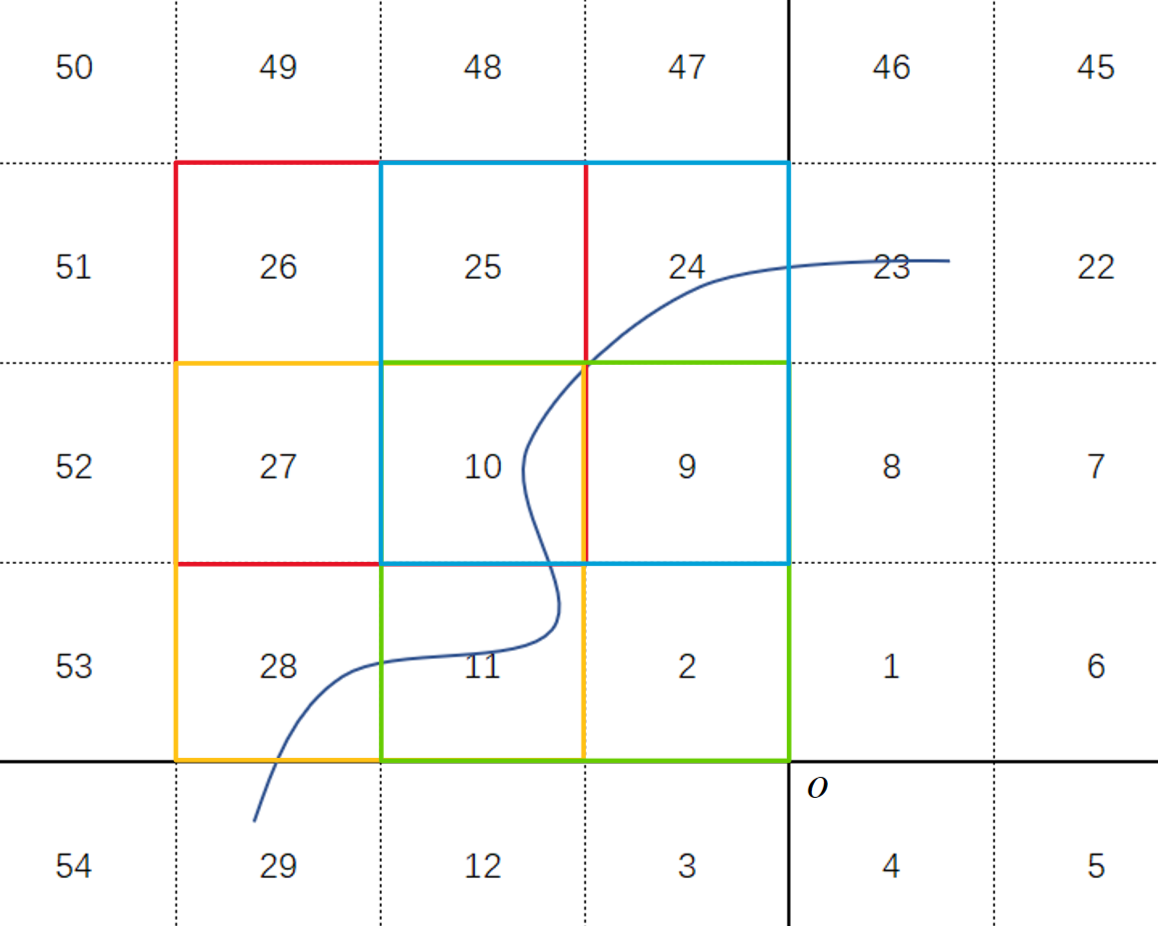
\includegraphics[width=0.7\textwidth]{figures/spatial_grid.png}
	\caption{网格划分方法}
	\note{注:在三维空间中采用逆时针螺旋方式进行网格划分的过程,通过实时更新相机位姿信息,处理四个相邻的网格以避免丢失重建空间。}
	\label{fig:spatial_grid}
\end{figure}

\par 在图\ref{fig:spatial_grid}中的原点处开始划分三维空间的网格。每个网格的序号按
逆时针螺旋形方式分配,与原点距离越近的网格序号越小。为了避免相机在运动过程中丢失重建空间,
系统在任何时刻都可以处理4个相邻的网格。图中,这四个网格被分
别标记为红色、蓝色、橙色和绿色区域。系统利用相机的实时位姿信息来确定每一帧图像的重建区域。
假设相机从29号网格开始向右上方移动,其在空间中的位置依次经过以(-2, 1), (-1, 1)和(-1, 2)为中心的网格。根据这些坐标点的位置,
可以确定系统当前需要处理的网格分别位于橙色、绿色和蓝色的区域。

\par 该网格划分方法大幅度减少了场景更新次数,从而提高了整个系统的运行效率。例如,在自动
驾驶系统中,如果汽车的速度为 12.5 m/s,每个网格的边长为 40 m,帧率为 30 帧/秒,那么在最快的情
况下,系统只需要每96帧(即每 3.2 秒)进行一次场景更新。

\par 该模块通过上述过程,在保证实时性和准确性的同时,实现了空间的有效划
分和数据的高效管理。通过位姿估计,可以获得相机的空间位置和朝向,从而定位场景和生成点云;
通过场景管理,可以进行动态场景重建,将重建范围扩大至无穷。